\documentclass[mathserif]{beamer}
\mode<presentation>
{
  \usetheme{Frankfurt}
  \setbeamercovered{transparent}
}

\setbeamertemplate{caption}[numbered]

\usepackage{bm}
\usefonttheme[onlymath]{serif}
\usepackage{mathrsfs}

\begin{document}


\title{Multiagent Bidirectionally-Coorinated Nets for Learning to Play StarCraft
Combat Games}

\author{Wenhao Yang
}
\institute{School of Mathematical Sciences

Peking University}
\begin{frame}
  \titlepage
\end{frame}

\date{}

\begin{frame}{Outline}
\tableofcontents
\end{frame}

\section{Models}
\begin{frame}{Setting}
  \begin{itemize}
    \item $N$ agents and $M$ opponents
    \item $S$ denotes the state space of the current game, shared among all the agents
    \item $A_{i}=A$ is the action space of the controlled agent $i$ for $i=1,2,...,N$
    \item $B_{i}=B$ is the action space of the enemy $i$ for $i=1,2,...,M$
    \item $T:S\times A^{N}\times B^{M}\rightarrow S$ is the deterministic transition function of the environment
    \item $R_{i}:S\times A^{N}\times B^{M}\rightarrow R$ is the reward function of agent/enemy $i$ for $i=1,2,...,N+M$
    \item $\bm{a}_{\theta}:S\rightarrow A^{N}$ is the deterministic of controlled agents
    \item $\bm{b}_{\phi}:S\rightarrow B^{M}$ is the deterministic of enemies
  \end{itemize}
\end{frame}
\subsection{Combat with Global Reward}
\begin{frame}{Combat with Global Reward}
\begin{itemize}
  \item Each agent in the same team shares the same reward
  \item Reward of Agents Definition:
  \begin{align}
    r(\bm{s},\bm{a},\bm{b})=\frac{1}{M}\sum_{j=N+1}^{M}\Delta R_{j}^{t}(\bm{s},\bm{a},\bm{b})-
    \frac{1}{N}\sum_{i=1}^{N}\Delta R_{i}^{t}(\bm{s},\bm{a},\bm{b})
  \end{align}
  where $\Delta R_{j}^{t}(\cdot)=R_{j}^{t-1}(\bm{s},\bm{a},\bm{b})-R_{j}^{t}(\bm{s},\bm{a},\bm{b})$
  \item Reward of Enemies is the opposite, making the sum of rewards from both camps euqlling to zero.
  \item Minimax game:
  \begin{align}
    Q^{*}(\bm{s},\bm{a},\bm{b})=r(\bm{s},\bm{a},\bm{b})+\lambda\max_{\theta}\min_{\phi}Q^{*}(\bm{s'},\bm{a}_{\theta}(\bm{s'}),\bm{b}_{\phi}(\bm{s'}))
  \end{align}
  where $\bm{s'}=\bm{s}^{t+1}$
\end{itemize}
\end{frame}
\subsection{Proposed Multiagent Actor-Critic with Individual Reward}
\begin{frame}{Proposed Multiagent Actor-Critic with Individual Reward}
  \begin{itemize}
    \item Considering team collaboration
    \item Each agent's local reward:
    \begin{align}
      r_{i}(\bm{s},\bm{a},\bm{b})=&\frac{1}{|j|}\sum_{j=N+1\bigcap\text{top-K(i)}}^{M}\Delta R_{j}(\bm{s},\bm{a},\bm{b})\\
      -&\frac{1}{|i'|}
      \sum_{i'=1\bigcap\text{top-K(i)}}^{N}\Delta R_{i'}(\bm{s},\bm{a},\bm{b})
    \end{align}
  \end{itemize}
\end{frame}

\begin{frame}{Model Architecture}
  \begin{figure}
    \centering
    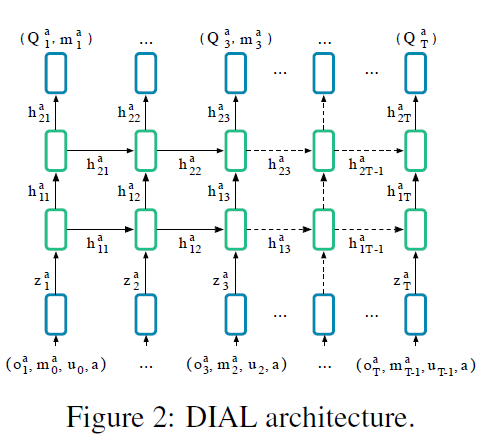
\includegraphics[scale=1]{fig/3}
  \end{figure}
\end{frame}

\begin{frame}{Model Architecture}
  \begin{itemize}
    \item Input: $(o_{t}^{a},m_{t-1}^{a'},u_{t-1}^{a},a)$
    \item Embedding:

    $z_{t}^{a}=f_{1}(o_{t}^{a})+f_{2}(m_{t-1})+f_{3}(u_{t-1}^{a})+f_{4}(a)$

    where $f_{1}$ is a task-specific network, $f_{2}$ is a 1-layer MLP and
    $f_{3}$ and $f_{4}$ are lookup tables
    \item 2-layer RNN with GRUs
    \item Output: $Q_{t}^{a},m_{t}^{a}$
  \end{itemize}
\end{frame}

\begin{frame}{Algorithm(DIAL)}
\begin{figure}'
  '
  \centering
  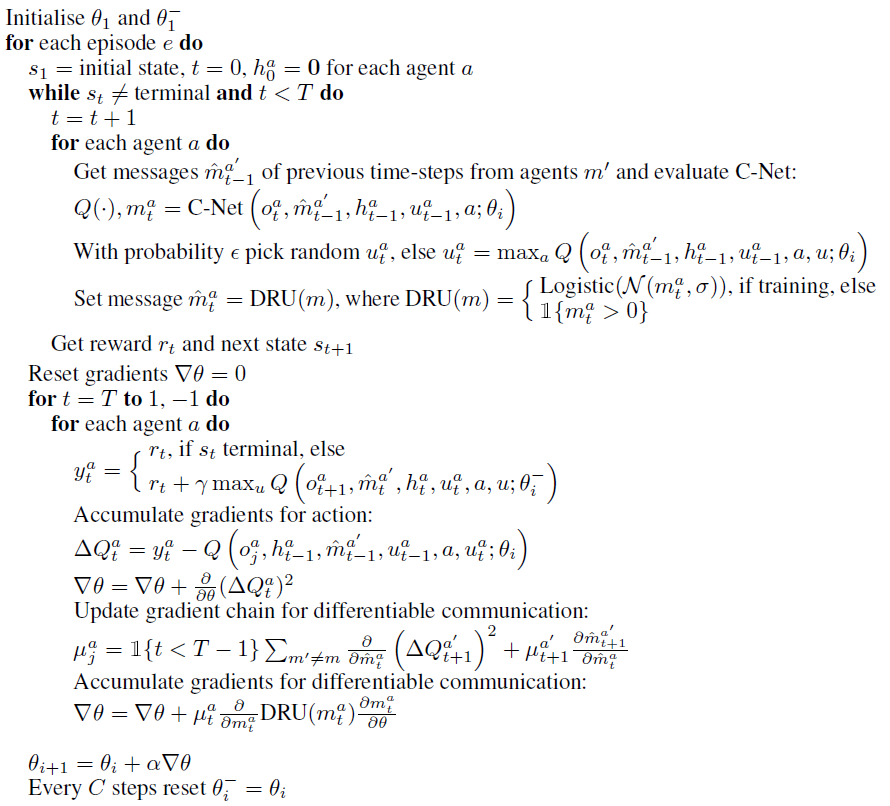
\includegraphics[scale=0.5]{fig/4}
\end{figure}
\end{frame}
\section{Experiments}
\subsection{Switch Riddle}
\begin{frame}{Experiment: Switch Riddle}
  \begin{figure}
    \centering
    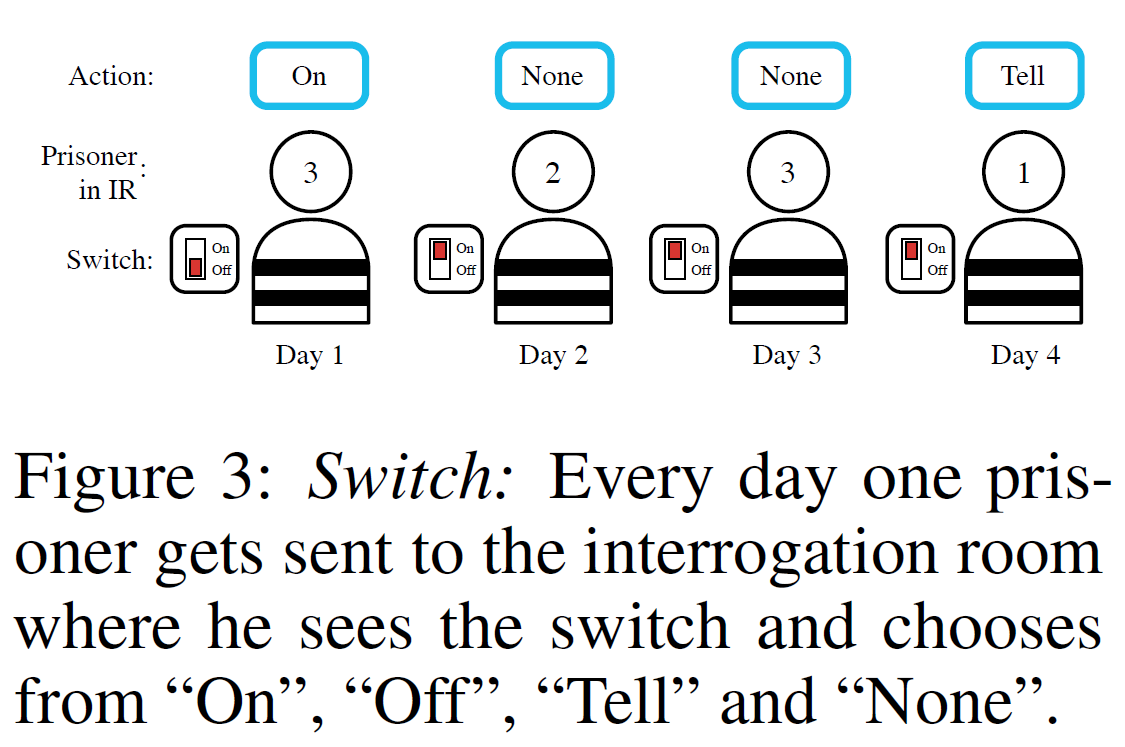
\includegraphics[scale=0.5]{fig/5}
  \end{figure}
\end{frame}

\begin{frame}{Experiment: Switch Riddle}
  \begin{itemize}
    \item $m_{t}^{a},o_{t}^{a}\in\{0,1\}$
    \item $u_{t}^{a}\in\{None,Tell\}$
    \item $r_{t}\in\{-1,0,1\}$
    \item Results:
    \begin{figure}
      \centering
      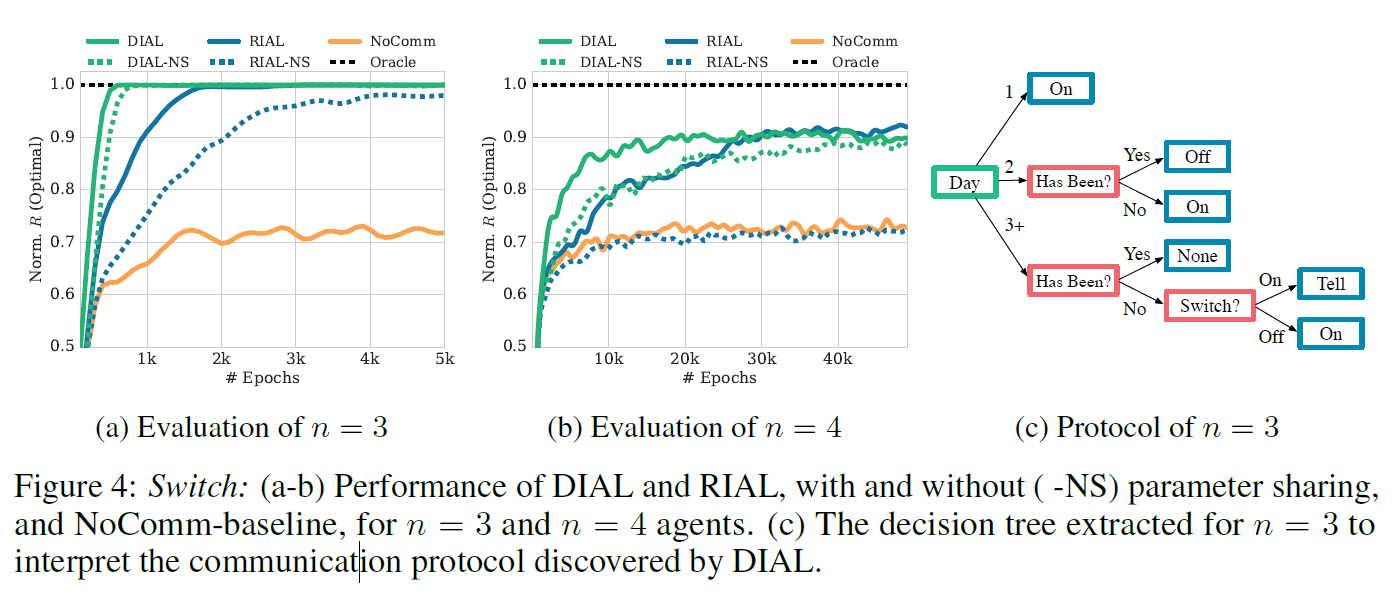
\includegraphics[scale=0.4]{fig/6}
    \end{figure}
  \end{itemize}
\end{frame}
\subsection{Multi-Step MNIST}
\begin{frame}{Experiment: Multi-Step MNIST}
  \begin{figure}
    \centering
    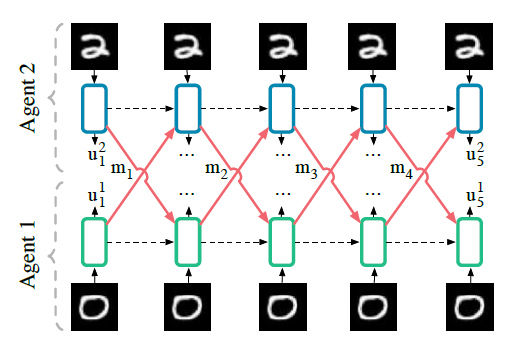
\includegraphics[scale=0.8]{fig/8}
  \end{figure}
\end{frame}
\subsection{Colour-Digit MNIST}
\begin{frame}{Experiment: Colour-Digit MNIST}
  \begin{figure}
    \centering
    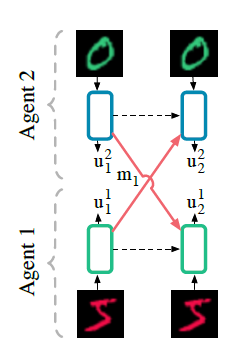
\includegraphics[scale=0.8]{fig/7}
  \end{figure}
  Not descriped clearly in paper
\end{frame}
\begin{frame}{MNIST results}
  \begin{figure}
    \centering
    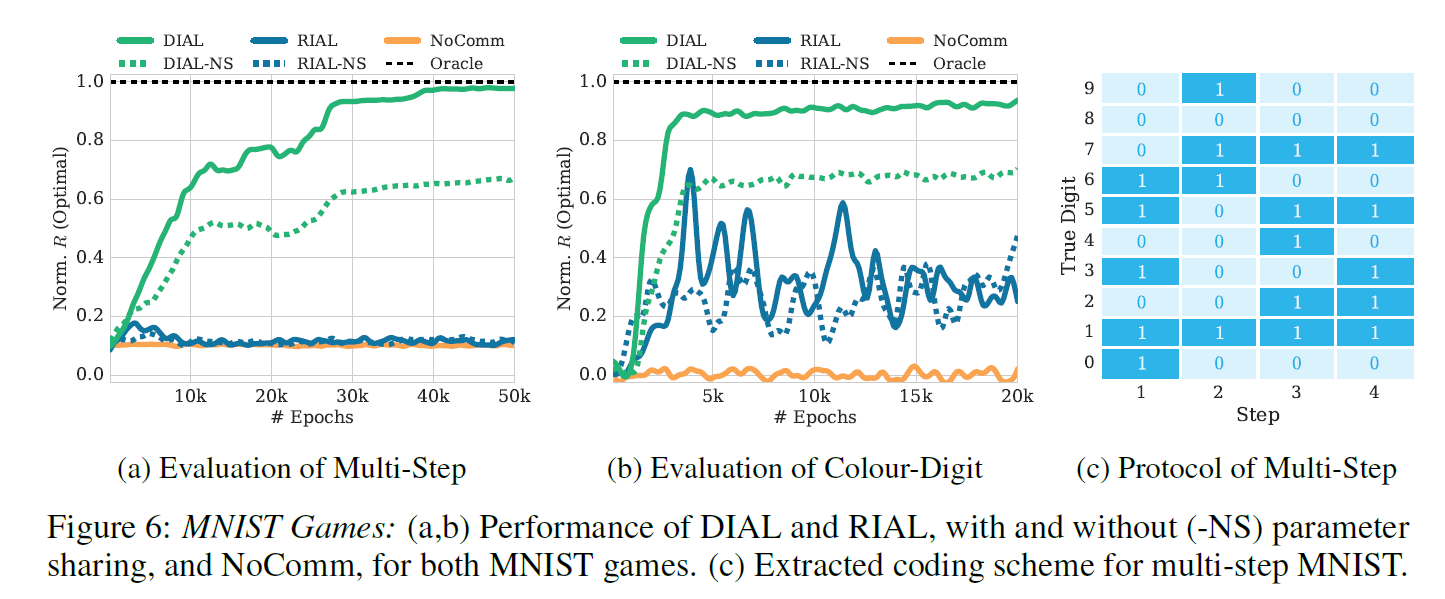
\includegraphics[scale=0.4]{fig/9}
  \end{figure}
\end{frame}
\section{Reference}
\begin{frame}{Reference}
  Reference:

  [1] Jakob N. Foerster, Yannis M. Assael, Nando de Freitas, Shimon Whiteson; Learning to Communicate with Deep Multi-Agent Reinforcement Learning
\end{frame}
\end{document}
